% generated by scripts/pkl_to_latex.py
% source PKL : vscan_v1_L8_Ne8_U10_t1_mode-uniform_nmin2_solver-gcg_full_restarts10_iter300_kmax5_tol1em09_V0to12_N25-ebabade1a2a1.pkl
% scan type  : vscan
% state      : gs
% quantity   : purity
% requires   : \usepackage{pgfplots} \pgfplotsset{compat=1.18}
% colours match the matplotlib PDF (tab10 cycle)
\definecolor{gmeC0}{HTML}{1F77B4}
\definecolor{gmeC1}{HTML}{FF7F0E}
\definecolor{gmeC2}{HTML}{2CA02C}
\definecolor{gmeC3}{HTML}{D62728}
\definecolor{gmeC4}{HTML}{9467BD}
\definecolor{gmeC5}{HTML}{8C564B}
\definecolor{gmeC6}{HTML}{E377C2}
\definecolor{gmeC7}{HTML}{17BECF}

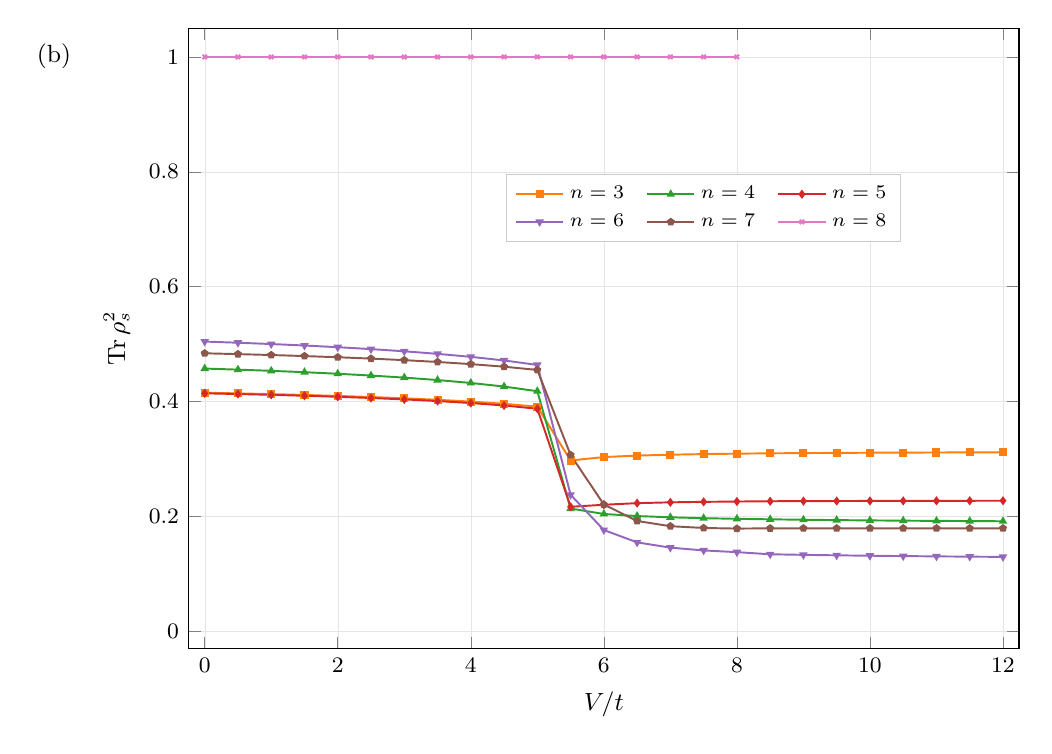
\begin{tikzpicture}
  \begin{axis}[
    width=\columnwidth,
    height=0.78\columnwidth,
    xlabel={$V/t$},
    ylabel={$\mathrm{Tr}\,\rho_s^2$},
    grid=both,
    grid style={line width=.1pt, draw=gray!20},
    tick label style={font=\footnotesize\rmfamily, /pgf/number format/fixed},
    label style={font=\small\rmfamily},
    scaled ticks=false,
    legend style={font=\scriptsize\rmfamily, draw=gray!40, at={(0.5,1.03)}, anchor=south, /tikz/every even column/.append style={column sep=6pt}},
    legend cell align={left},
    legend columns=3,
    ymin=-0.03,
    ymax=1.05,
    xmin=-0.24,
    xmax=12.24,
    legend style={at={(0.620,0.710)}, anchor=center, fill=white},
    after end axis/.append code={\node[anchor=east, font=\small\rmfamily] at (axis description cs:-0.13,0.954) {(b)};},
  ]
    \addplot[color=gmeC1, mark=square*, mark size=1.1pt, line width=0.7pt] coordinates {
        (0,0.415247) (0.5,0.414107) (1,0.41282) (1.5,0.41136)
        (2,0.409694) (2.5,0.407778) (3,0.405555) (3.5,0.402944)
        (4,0.399819) (4.5,0.39597) (5,0.390975) (5.5,0.297223)
        (6,0.303211) (6.5,0.305754) (7,0.30731) (7.5,0.308371)
        (8,0.309135) (8.5,0.309709) (9,0.310143) (9.5,0.310483)
        (10,0.310755) (10.5,0.310976) (11,0.311157) (11.5,0.311308)
        (12,0.311435)
    };
    \addlegendentry{$n=3$}
    \addplot[color=gmeC2, mark=triangle*, mark size=1.1pt, line width=0.7pt] coordinates {
        (0,0.457304) (0.5,0.455451) (1,0.453359) (1.5,0.450986)
        (2,0.448278) (2.5,0.445166) (3,0.441557) (3.5,0.437317)
        (4,0.432243) (4.5,0.425988) (5,0.417868) (5.5,0.213541)
        (6,0.204084) (6.5,0.200467) (7,0.198293) (7.5,0.196768)
        (8,0.195616) (8.5,0.194789) (9,0.194033) (9.5,0.193408)
        (10,0.192883) (10.5,0.192434) (11,0.192047) (11.5,0.191708)
        (12,0.191409)
    };
    \addlegendentry{$n=4$}
    \addplot[color=gmeC3, mark=diamond*, mark size=1.1pt, line width=0.7pt] coordinates {
        (0,0.414191) (0.5,0.412954) (1,0.411556) (1.5,0.409967)
        (2,0.408151) (2.5,0.406058) (3,0.403622) (3.5,0.400749)
        (4,0.397291) (4.5,0.392996) (5,0.387359) (5.5,0.216603)
        (6,0.220148) (6.5,0.222929) (7,0.224366) (7.5,0.225206)
        (8,0.225749) (8.5,0.226256) (9,0.22648) (9.5,0.226653)
        (10,0.22679) (10.5,0.226898) (11,0.226986) (11.5,0.227057)
        (12,0.227115)
    };
    \addlegendentry{$n=5$}
    \addplot[color=gmeC4, mark=triangle*, mark size=1.1pt, mark options={rotate=180}, line width=0.7pt] coordinates {
        (0,0.504323) (0.5,0.5023) (1,0.500023) (1.5,0.497451)
        (2,0.494533) (2.5,0.491204) (3,0.487379) (3.5,0.482944)
        (4,0.477729) (4.5,0.471458) (5,0.463612) (5.5,0.237552)
        (6,0.176153) (6.5,0.154641) (7,0.145457) (7.5,0.140599)
        (8,0.137605) (8.5,0.133902) (9,0.132907) (9.5,0.132074)
        (10,0.131367) (10.5,0.13076) (11,0.130233) (11.5,0.129772)
        (12,0.129364)
    };
    \addlegendentry{$n=6$}
    \addplot[color=gmeC5, mark=pentagon*, mark size=1.1pt, line width=0.7pt] coordinates {
        (0,0.483894) (0.5,0.482482) (1,0.480889) (1.5,0.479083)
        (2,0.477027) (2.5,0.474673) (3,0.471956) (3.5,0.468792)
        (4,0.465057) (4.5,0.460553) (5,0.454915) (5.5,0.306886)
        (6,0.220591) (6.5,0.191909) (7,0.182804) (7.5,0.17972)
        (8,0.178637) (8.5,0.179104) (9,0.179125) (9.5,0.179141)
        (10,0.179152) (10.5,0.17916) (11,0.179165) (11.5,0.179167)
        (12,0.179168)
    };
    \addlegendentry{$n=7$}
    \addplot[color=gmeC6, mark=x, mark size=1.1pt, line width=0.7pt] coordinates {
        (0,1) (0.5,1) (1,1) (1.5,1)
        (2,1) (2.5,1) (3,1) (3.5,1)
        (4,1) (4.5,1) (5,1) (5.5,1)
        (6,1) (6.5,1) (7,1) (7.5,1)
        (8,1)
    };
    \addlegendentry{$n=8$}
  \end{axis}
\end{tikzpicture}
